%%
% This is an Overleaf template for presentations
% using the TUM Corporate Desing https://www.tum.de/cd
%
% For further details on how to use the template, take a look at our
% GitLab repository and browse through our test documents
% https://gitlab.lrz.de/latex4ei/tum-templates.
%
% The tumbeamer class is based on the beamer class.
% If you need further customization please consult the beamer class guide
% https://ctan.org/pkg/beamer.
% Additional class options are passed down to the base class.
%
% If you encounter any bugs or undesired behaviour, please raise an issue
% in our GitLab repository
% https://gitlab.lrz.de/latex4ei/tum-templates/issues
% and provide a description and minimal working example of your problem.
%%


\documentclass[
  german,            % define the document language (english, german)
  aspectratio=169,    % define the aspect ratio (169, 43)
  % handout=2on1,       % create handout with multiple slides (2on1, 4on1)
  % partpage=false,     % insert page at beginning of parts (true, false)
  % sectionpage=true,   % insert page at beginning of sections (true, false)
]{tumbeamer}


% load additional packages
\usepackage{booktabs}
\usepackage{graphicx}
\usepackage{tikz}
\usepackage{url}
\usepackage{pgfplots}
\usepackage{hyperref}
\usepackage{pmboxdraw}
\usepackage{float}
\usepackage{babel}[ngerman]
\usepackage{csquotes}[autostyle]
\usepackage[useregional]{datetime2}

% image path
\graphicspath{ {./resources/} }

% presentation metadata
\title{Übung 04: x86-Assembly}
\subtitle{Grundlagenpraktikum Rechnerarchitektur}
\author{Niklas Ladurner}

\institute{\theChairName\\\theDepartmentName\\\theUniversityName}
\date{\DTMdisplaydate{2024}{5}{10}{-1}}

\footline{\insertauthor~|~\insertshorttitle~|~\insertshortdate}


% macro to configure the style of the presentation
\TUMbeamersetup{
  title page = TUM tower,         % style of the title page
  part page = TUM toc,            % style of part pages
  section page = TUM toc,         % style of section pages
  content page = TUM more space,  % style of normal content pages
  tower scale = 1.0,              % scaling factor of TUM tower (if used)
  headline = TUM threeliner,      % which variation of headline to use
  footline = TUM default,         % which variation of footline to use
  % configure on which pages headlines and footlines should be printed
  headline on = {title page},
  footline on = {every page, title page=false},
}

% available frame styles for title page, part page, and section page:
% TUM default, TUM tower, TUM centered,
% TUM blue default, TUM blue tower, TUM blue centered,
% TUM shaded default, TUM shaded tower, TUM shaded centered,
% TUM flags
%
% additional frame styles for part page and section page:
% TUM toc
%
% available frame styles for content pages:
% TUM default, TUM more space
%
% available headline options:
% TUM empty, TUM oneliner, TUM twoliner, TUM threeliner, TUM logothreeliner
%
% available footline options:
% TUM empty, TUM default, TUM infoline


\begin{document}

\maketitle

\begin{frame}[c]{}{}
  \begin{center}
    \LARGE  Keine Garantie für die Richtigkeit der Tutorfolien: Bei Unklarheiten/Unstimmigkeiten
    haben VL-Folien Recht!
  \end{center}
\end{frame}

\begin{frame}[c, fragile]{Organisatorisches}{}
  \begin{itemize}
    \item Für den ASM-Teil wird wieder die alte Praktikumswebsite verwendet (siehe Links)
    \item Anmeldung mit eurer TUM-Kennung (gxXXxxx)
    \item noch 4 Wochen mit Aufgaben, danach Projektphase
    \item Notenbonus-Grenze von 75\% wird über \textit{alle} Wochen hinweg berechnet
  \end{itemize}
\end{frame}

\begin{frame}[c, fragile]{x86-64 Basics}{}
  \begin{itemize}
    \item CISC-Architektur, 64 Bit (8 Byte Register), weit verbreitet
    \item nur 16 GP-Register!
    \item 32 Bit sign extended Immediates (mov verwendet 64 Bit!)
    \item kein Unterschied zwischen Instruktionsbezeichnungen für reg/reg vs reg/imm wie in RISC-V
    \item Aufteilung der Register in Teilregister (8B, 4B, 2B, 1B, 1B):
          \begin{center}
            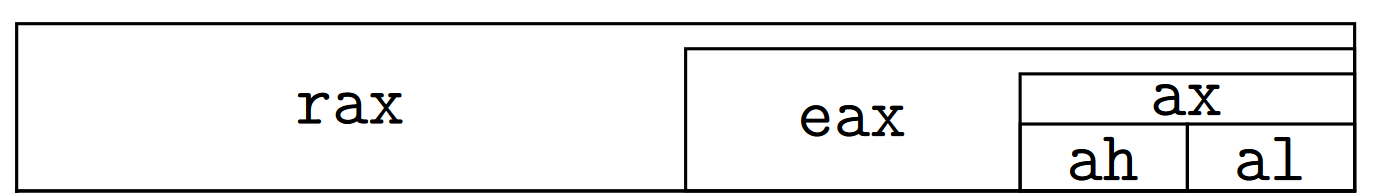
\includegraphics[width=0.7\textwidth]{w04_reg_div.png}
          \end{center}
    \item Schreiben von 4B-Register löscht obere Bits!
  \end{itemize}
\end{frame}

\begin{frame}[c, fragile]{Grundlegende Befehle}{}
  \begin{itemize}
    \item \verb|mov dst, src|
    \item \verb|add/sub dst, src| (erster Operand sowohl src als auch dst)
    \item arithmetische Operationen setzen Flags, Sprünge/Branches überprüfen Flag-Register
    \item \verb|cmp| entspricht \verb|sub|, setzt aber nur Flags
    \item \verb|test| entspricht \verb|and|, setzt aber nur Flags
    \item Speicherzugriff (explizite Größenangabe): \verb|add dword ptr [rax], 1|
    \item Warum funktioniert \verb|mov eax, [edx]| ohne explizite Zugriffsgröße?
  \end{itemize}
\end{frame}

\begin{frame}[c, fragile]{Stack}{}
  \begin{itemize}
    \item kein explizites Schreiben an sp wie in RISC-V notwendig
    \item \verb|push|, \verb|pop| ändert sp automatisch
    \item Rücksprungadresse wird auch automatisch abgespeichert/wiederhergestellt: \verb|call| und \verb|ret|
    \item 16-Byte-Alignment vor Funktionsaufrufen wie in RISC-V
  \end{itemize}
\end{frame}

\begin{frame}[c]{}{}
  \begin{center}
    \LARGE Fragen?
  \end{center}
\end{frame}

\begin{frame}[fragile, c]{Links}{}
  \begin{itemize}
    \item Zulip: \href{https://zulip.in.tum.de/#narrow/stream/2267-GRA-Tutorium---Gruppe-20}{\enquote{GRA Tutorium - Gruppe 20}}
          bzw. \href{https://zulip.in.tum.de/#narrow/stream/2269-GRA-Tutorium---Gruppe-22}{\enquote{GRA Tutorium - Gruppe 22}}
    \item \href{https://gra.caps.in.tum.de}{\enquote{Praktikumswebsite}}
    \item \href{https://www.felixcloutier.com/x86/}{x86 instruction reference by Félix Cloutier}
    \item \href{https://graphics.stanford.edu/~seander/bithacks.html#CountBitsSetParallel}{Bit Hacks}
    \item \href{https://flint.cs.yale.edu/cs421/papers/x86-asm/asm.html}{x86 ASM Guide}
  \end{itemize}
\end{frame}

\maketitle

\end{document}
